\documentclass{article}
\usepackage[margin=3cm]{geometry}
\usepackage{amsmath, amssymb, amsthm}
\usepackage{graphicx}
\usepackage[utf8]{inputenc} 
\usepackage[T1]{fontenc} 
\usepackage{csquotes} 
\usepackage[hidelinks]{hyperref} 
\usepackage[style=ieee, backend=biber]{biblatex} 
\usepackage{minted}

% \addbibresource{references.bib}

\title{INF264 - Project 1 report}
\author{Julian Hamre}
\date{September 2026}

\begin{document}

\maketitle
\tableofcontents
\newpage

\section{Introduction}

In this project, I implemented the ID3 decision tree classifier algorithm from scratch.
This machine learning model classifies data points by traversing through a binary tree.
The tree consists of nodes containing routing logic based on specific features of the data point.
These nodes guide each data point to its most appropriate decision-making leaf.
The leaf returns a label which classifies the data point.
My implementation is used to generalize the given churn dataset 
and evaluated using several classifier metrics.
I have completed this project alone.

\section{Implementation}

The classifier is represented by the \texttt{DecisionTreeClassifier} class
located in \texttt{decision\_tree\_classifier.py}. This class constructs and utilizes a
\texttt{DecisionTree} object during training and predicting.

\subsection{The \texttt{DecisionTree} class}

A \texttt{DecisionTree} object represents a binary tree of nodes.
It does not contain references to all the nodes in the tree explicitly.
It only contains a reference to its root node. 
This is because the nodes themselves contain references to their nearest neighbors,
enabling traversal between them. 
New nodes are added to the tree with the two child assigning methods.
These take a to-become-parent node and a to-become-child node as input arguments,
assign the parent node as the child nodes' parent reference, and vice versa.

\subsubsection{Nodes}

A \texttt{Node} object is essentially a terminal for traversing data points.
It contains a reference to its parent node, left child node, and right child node, if they exist.
The node's depth in the tree is also stored in the object, 
and is calculated by adding one to the parent node's depth value.
Additionally, a node can contain a decision, which is the label value it will return
to classify a data point.
However, the node will only return the decision if it is a leaf in the tree.
Otherwise, its job is to route a data point further downwards in the tree
using its assigned \texttt{Router} object.

\subsubsection{Routers}

A \texttt{Router} object's main job is to select the next node in the path of a traversing data point.
Each router decides if a data point should continue to the left or right child node
based on a single feature of the point.
I have implemented two \texttt{Router} classes, one for routing based on categorical features,
and one for routing based on numerical (continuous) features.
These two classes extend the same superclass, which implements their common logic.

The reason I chose to implement two classes, is because it is beneficial to binarize categorical
and numerical variables differently.\footnote{I am aware that the project description said that I could assume all features were numerical (continuous). However, I chose to distinguish between numerical and categorical features to enable better model performance}
If the router routes based on a categorical feature,
it should go either left or right based on if the feature value in question is,
or is not equal to a certain value. 
For example, if you had a feature called weather, you could check if it was sunny or not sunny.
Here is my implementation of that method.

\begin{minted}{python}
def route(self, datapoint, from_node):
    feature_value = datapoint[self._feature_col]
    if feature_value == self.__threshold:
        return from_node.right_child()
    else:
        return from_node.left_child()
\end{minted}

Positives are always associated with going right. 
So, if the data point's feature value is equal to the certain value, called the threshold,
it will be routed to the right child node. Otherwise, it will be routed left.

This is not a sensible approach for numerical features,
because most of them are unique.
Every unique feature value would then get its own split in the tree.
Therefore, a \texttt{NumericalRouter} object routes a data point to the right
if its feature value is bigger than the mean feature value of the data the router was trained on.
Otherwise, it will be routed left.

\begin{minted}{python}
if feature_value <= self.__threshold:
    return from_node.left_child()
else:
    return from_node.right_child()
\end{minted}

A router also contains logic for dividing and routing training dataset partitions during tree growth,
which I will explain under \emph{Data splitting} in Section~\ref{sec:the-trainingdata-class}.

\subsection{Training}

Model training consists of growing the decision tree.
This is mostly handled by a \texttt{TreeGrower} object constructed by the \texttt{fit} method of the \texttt{DecisionTreeClassifier}.
However, data management and information gain calculation are handled
by helper classes.

\subsubsection{The \texttt{TrainingData} class}
\label{sec:the-trainingdata-class}

I use \texttt{TrainingData} objects to represent the training dataset partitions during model training.
These objects have several essential methods used by the tree grower, like \texttt{features\_are\_equal} for checking if all feature rows are equal,
or the \texttt{feature\_values} method, which can retrieve the feature values given a feature column index. 
Their most important responsibilities, however, are to distinguish between feature variable types and to perform data splitting.

\paragraph{Distinguishing between feature types.}
A \texttt{TrainingData} object always keeps track of which features are categorical and numerical.
This is not straight forward, because I represent the features and labels using numpy matrices.
Numpy matrices can only contain one datatype, so I have no way to determine the feature types using the matrices.
Therefore, I predetermine the feature types using the static class method \texttt{create\_from\_pandas\_data}.
This method receives the training data represented by pandas dataframes.
It checks all the column dtypes and stores the indices of the columns
containing floating point numbers in a list.
Finally, it passes on this list to a \texttt{TrainingData} object.

This enables categorical features to be returned as a column of integers, and numerical features as a column of floats.
Also, a node can use the \texttt{is\_numerical\_feature} method to select the appropriate router type for the node.

\paragraph{Data splitting.}
A \texttt{TrainingData} object can split itself in two partitions using the \texttt{divided\_data} method.
The method does this using a row masking function passed to it as an argument.
This function returns a boolean matrix constructed based on a given feature column.
For example if the feature was weather again,
the boolean matrix can contain \texttt{True} for each row containing \texttt{"sunny"},
and \texttt{False} for every other row.
Thus, the \texttt{TrainingData} object can construct two new \texttt{TrainingData} objects,
where one contains all the rows aligning with the \texttt{False} values,
and the other contains the rows aligning with the \texttt{True} ones.
The list containing the column indices of the numerical features is also passed on to the two partitions,
ensuring that they still can distinguish between feature types.

The actual call to the \texttt{divided\_data} method happens inside a \texttt{Router} object,
because it is the router that contains the row masking function implementation.
The routers calculate the boolean values of the mask based on how they would route each row as a datapoint.
Rows that would have been routed left get \texttt{False} values,
and rows that would have been routed right get \texttt{True} values.

\subsubsection{Information gain calculation}

\paragraph{The \texttt{PurityIndex} class.}
This class can calculate the purity $I(Y)$ of a label column $Y$ using either the entropy or gini index.
Both purity representations are sums of terms $t(y_i)$ for each unique label $y_i$ $Y$ can take.

\begin{align*}
  I(Y) = \sum_{i=0}^{n}t(y_i)
\end{align*}

It is the $t(y_i)$ terms that differ between the entropy and gini index.

\begin{align*}
  t_{\text{entropy}}(y_i) &= - P(Y = y_i) \log_2 P(Y = y_i)\\ 
  t_{\text{gini}}(y_i) &= P(Y = y_i)(1 - P(Y = y_i))
\end{align*}

Therefore, I implemented one method for each term.

\begin{minted}{python}
def __entropy_term(self, probability):
    return -probability * np.log2(probability) 

def __gini_term(self, probability):
    return probability * (1 - probability)
\end{minted}

Then, during object construction, the object's \texttt{calculate} method is determined
as the sum of terms using the term function aligning with the given keyword argument 
\texttt{index\_type}. The probability $P(Y = y_i)$ for each unique label $y_i$ is calculated as
the number of times the label appears in the column over the total number of labels.

\paragraph{The \texttt{InformationGain} class.}
I use the \texttt{InformationGain} class to find the feature column $X$ with the highest information gain.
It does that by comparing the information gain score $IG(X) = I(Y) - I(Y | X)$ of each feature column.
The scores are calculated using the purity scores given by a \texttt{PurityIndex} object.
I had to implement two different information gain calculators, one for categorical feature columns,
and one for numerical ones.
This is because conditional purity of a label column $Y$ is calculated differently given a numerical feature $X$.

\begin{align*}
  I_{\text{categorical feature}} (Y|X) &= \sum_i P(X = x_i) I(Y|X = x_i)\\ 
  I_{\text{numerical feature}}(Y|X) &= P(X \leq \bar{X}) I(Y | X \leq \bar{X}) + P(X > \bar{X}) I(Y | X > \bar{X})   
\end{align*}

For a numerical feature, the sum only contains two terms.
One considering the labels of the features that are smaller than the mean feature value $\bar{X}$,
and one considering the labels of the features that are larger.

\subsubsection{The \texttt{TreeGrower} class}

This class brings all the model training logic together.
The growth process is started by calling the \texttt{grow\_tree} method on the \texttt{TreeGrower} object.
This method takes a \texttt{TrainingData} object as an input argument, and makes the first call to
the private \texttt{grow\_from} method on the root node.

\begin{minted}{python}
def __grow_from(self, node, data):
    if data.labels_are_equal() or data.features_are_equal():
        self.__complete_leaf(node, data)
        return
    information_gain = InformationGain(data, purity_index=self.__criterion)
    best_feature_col = information_gain.feature_with_highest_information_gain()
    self.__complete_subtree(node, best_feature_col, data)
\end{minted}

This is the method that contains the ID3 algorithm.
Firstly, it does the equality checks on the labels and features to decide if the node should become a leaf.
If not, it splits on the feature with the highest information gain.
The splitting is done by calling the \texttt{complete\_subtree} method.
This method completes the node by adding its decision as the majority label, and appropriate router
object based on the selected feature. It also checks if the maximum tree depth has been
reached, and leaves the node as a leaf if it has.
Otherwise, it will create branches based on how the router splits on the feature.

The branching is done by the \texttt{branch\_from} helper method.
It creates two new child nodes and attaches them to the node branched from.
The data is then split in two using the node's router, and each child node
gets one data partition each.
Thereafter, the \texttt{grow\_grom} method is usually recursively called on the child nodes for continued growth. 
However, if the feature that was split on was a multicategorical feature, the algorithm
will forcibly re-split on the same feature, until no data partitions contain more than one instance of that feature.
This is done to emulate what would have been a multibranch split in a non-binary tree.

\subsection{Predicting}

The prediction process is the simplest part of the implementation.
The \texttt{predict} method of the \texttt{DecisionTreeClassifier} iterates through 
the rows of a pandas dataframe of feature values to be predicted.
It calls the recursive \texttt{decision} method on each row, which traverses it through the decision tree.
The path is made by calling the \texttt{route} method of each node it encounters.
The router in each node returns the next node based on the row's instance
of the feature the router was trained on.
When a leaf is reached, it returns the decision label.
The predicted labels are added to a list and returned as an array.

\section{Model evaluation}

\subsection{Approach}

\paragraph{Performance measure.}
I evaluated my model on the given churn dataset.
This is an unbalanced dataset, because only 27 \% of the train samples are labeled as \textit{churn}.
Therefore, the accuracy score might be a bad approach, 
since a baseline model predicting \textit{no churn} for each sample would get a 73 \% accuracy score.
That is why I chose the F1 score, because it optimizes based on both precision and recall.
These metrics both focus on the number of predicted \textit{churn} values as a fraction of a total.

\paragraph{Hyperparameters.}
I had two hyperparameters available for tuning,
which were \texttt{criterion} and \texttt{max\_depth}.
\texttt{criterion} is a binary variable, which makes it easy to select values for it.
The good candidate values for \texttt{max\_depth}, however, were not immediately obvious.
Therefore, I started by choosing a wide spread of depth limits before narrowing
it down after getting my first validation scores.

\paragraph{Model selection.}
I chose to use $k$-fold validation as the model selection method,
which enabled me to evaluate a mean cross-validated F1 score for each model.
Thus, I was able to use as much of my dataset as possible for training, and avoid
unlucky train-validation-splits. With $k = 5$, I kept the validation partition
big enough to remain reliable, since the label distribution was unbalanced.
After having evaluated a number of models, the one with the highest score could
be selected, and finally be tested using the unseen test data, ensuring an unbiased final 
evaluation of the model.

Random seeds were consistently used whenever any step in the training process was done using randomizing. 
This ensured result reproducibility.

\subsection{Result}

\subsubsection{Performance} 

I ran both my own implementation and the Sklearn implementation through the same model selection
procedure to enable a comparison between their performances.
During model training, the different models received relatively similar mean cross-validated F1 scores for the different hyperparameter values,
see \autoref{fig:val-scores}.
Models using the \texttt{entropy} criterion performed almost identically to the models using the \texttt{gini} criterion,
so I only included the figure showing the entropy validation scores.

\begin{figure}[ht]
  \centering
  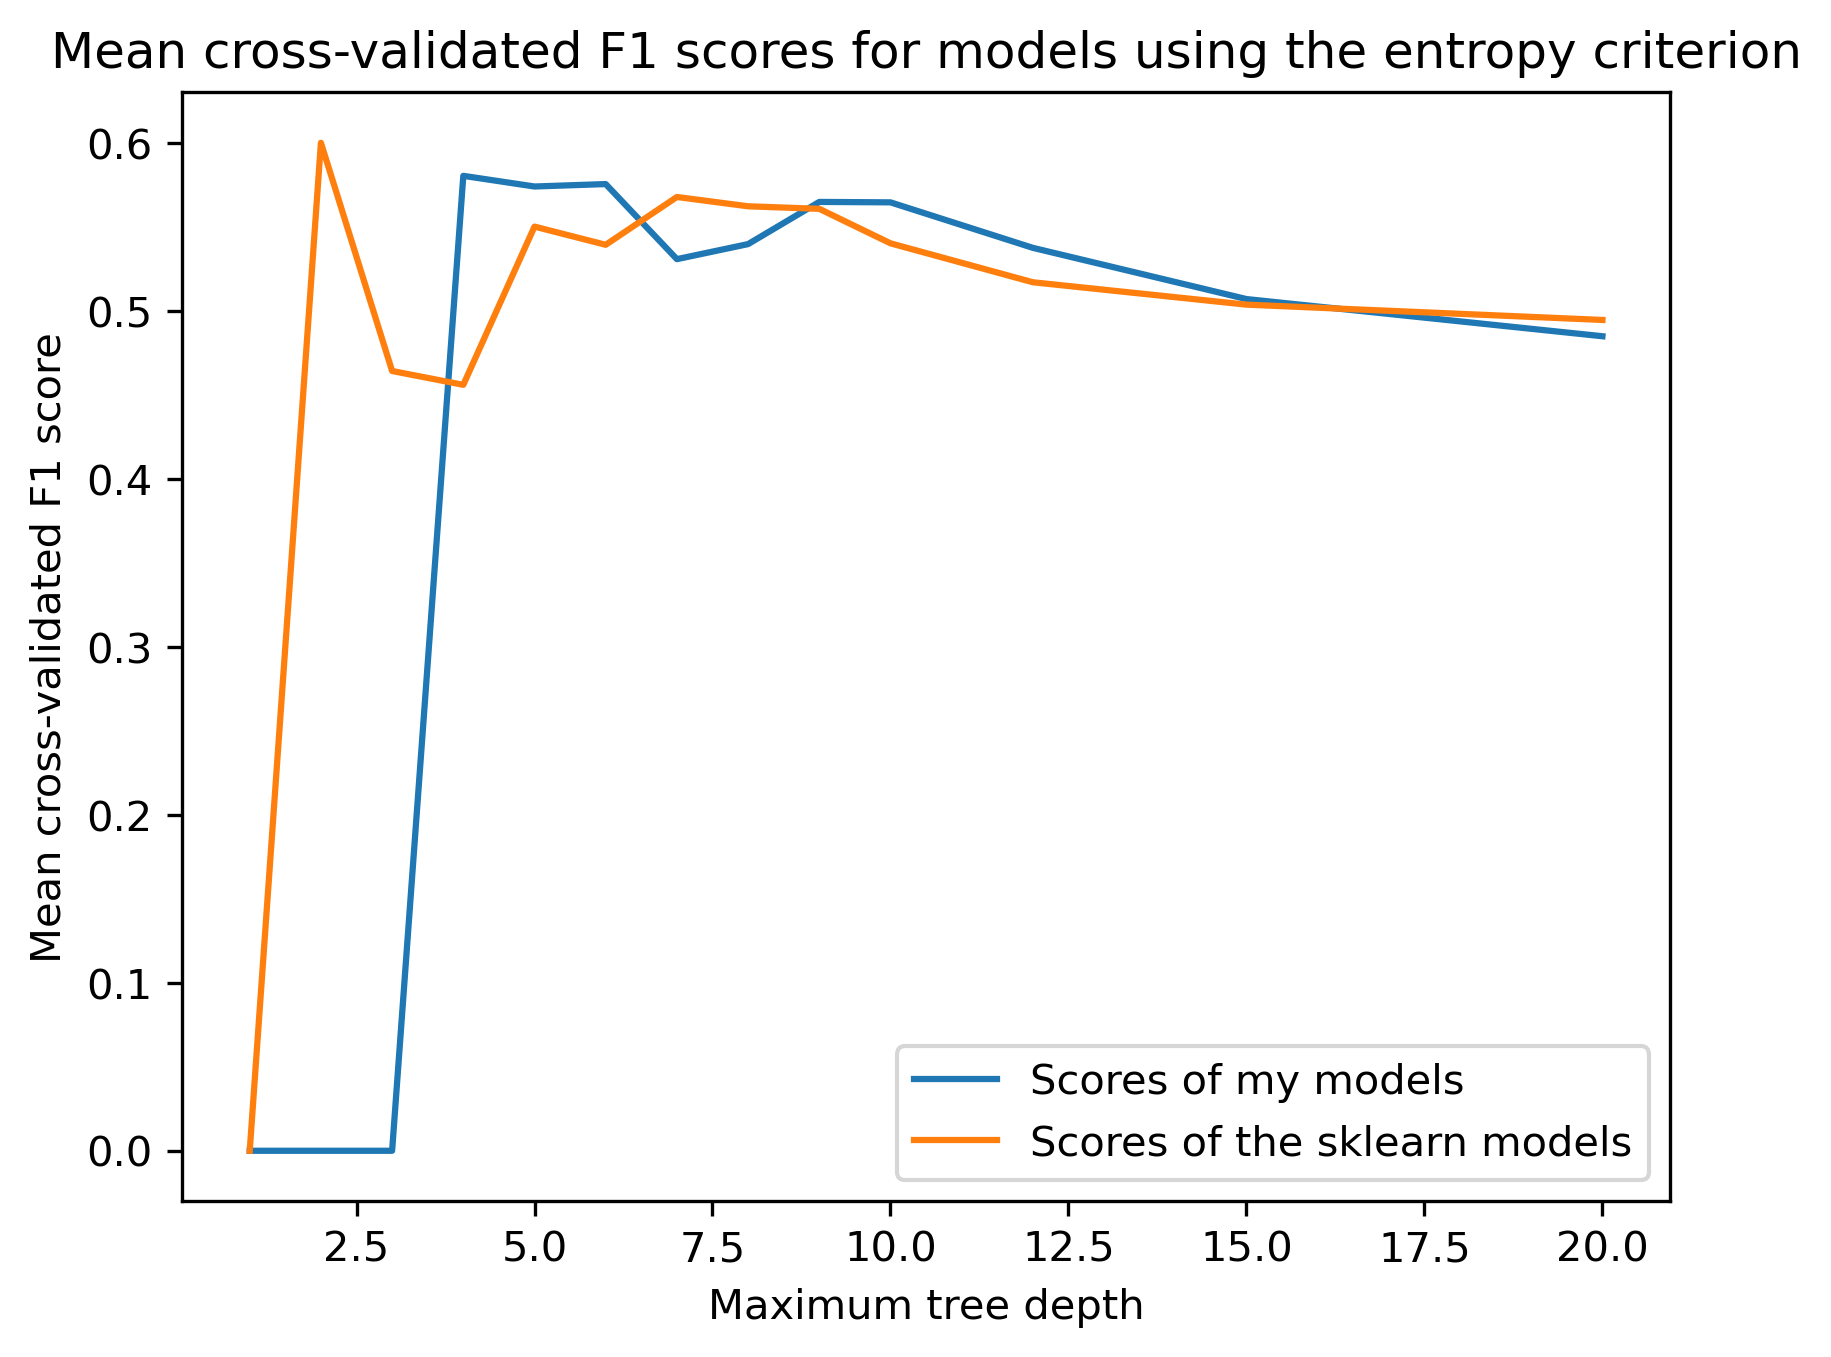
\includegraphics[width=0.8\textwidth]{figures/cross-val-scores-entropy.png}
  \caption{Mean cross-validated F1 scores of models using the entropy criterion}
  \label{fig:val-scores}
\end{figure}

\begin{table}[htb]
  \centering
  \begin{tabular}{lccc}
    \hline
    Implementation & Criterion & Max depth & Mean cross-validated F1 score \\
    \hline
    My own & Entropy & 4 & 0.581 \\
    \hline
    Sklearn & Entropy & 2 & 0.600 \\
    \hline
  \end{tabular}
  \caption{Characteristics of the selected models}
  \label{tab:selected-models}
\end{table}

The selected models' characteristics are described in \autoref{tab:selected-models}.
My model received a mean cross-validated F1 score of 0.581.
This outperforms the baselines predicting a constant label value.
By the definition of the F1 score, the baseline predicting \textit{no churn} only
will get score 0, because it predicts zero positives.
If I evaluate a baseline only predicting \textit{churn} on my training dataset,
I will get this F1 score.

\begin{align*}
  F1_{\text{only churn}}= 2\cdot\frac{\text{precision}\cdot\text{recall}}{\text{precision} + \text{recall}}
     \approx 2\cdot\frac{0.27\cdot 1}{0.27 + 1}  
     = 0.425 
\end{align*}


After the models were selected, I could finally test them using test data.
Their scores are described in \autoref{tab:test-performances}.
They show that my implementation has a slightly better accuracy,
precision and F1 score than Sklearn's implementation, but falls behind on recall.
All in all, they have similar performances.

\begin{table}[htb]
  \centering
  \begin{tabular}{lcccc}
    \hline
    Implementation & Accuracy & Precision & Recall & F1 score \\
    \hline
    My own & 0.771 & 0.565 & 0.605 & 0.584 \\
    \hline
    Sklearn & 0.743 & 0.514 & 0.655 & 0.576 \\
    \hline
  \end{tabular}
  \caption{Performances on the test dataset}
  \label{tab:test-performances}
\end{table}

\subsubsection{Feature importance}

I implemented the permutation importance algorithm to determine the features that
have the most influence on the predictions. 
This algorithm scores a feature based on how much the model performance changes
when the feature is scrambled in the dataset to be predicted. 
The permutation score is defined as the mean deviation from the model's reference score,
which is the model performance on the untouched dataset.
I ran this algorithm on my model using test data and the accuracy score performance metric.
Only two features received a non-zero permutation score.
\texttt{InternetService} was scored 0.0619, and \texttt{Contract} was scored 0.0739.

\begin{figure}[htb]
  \centering
  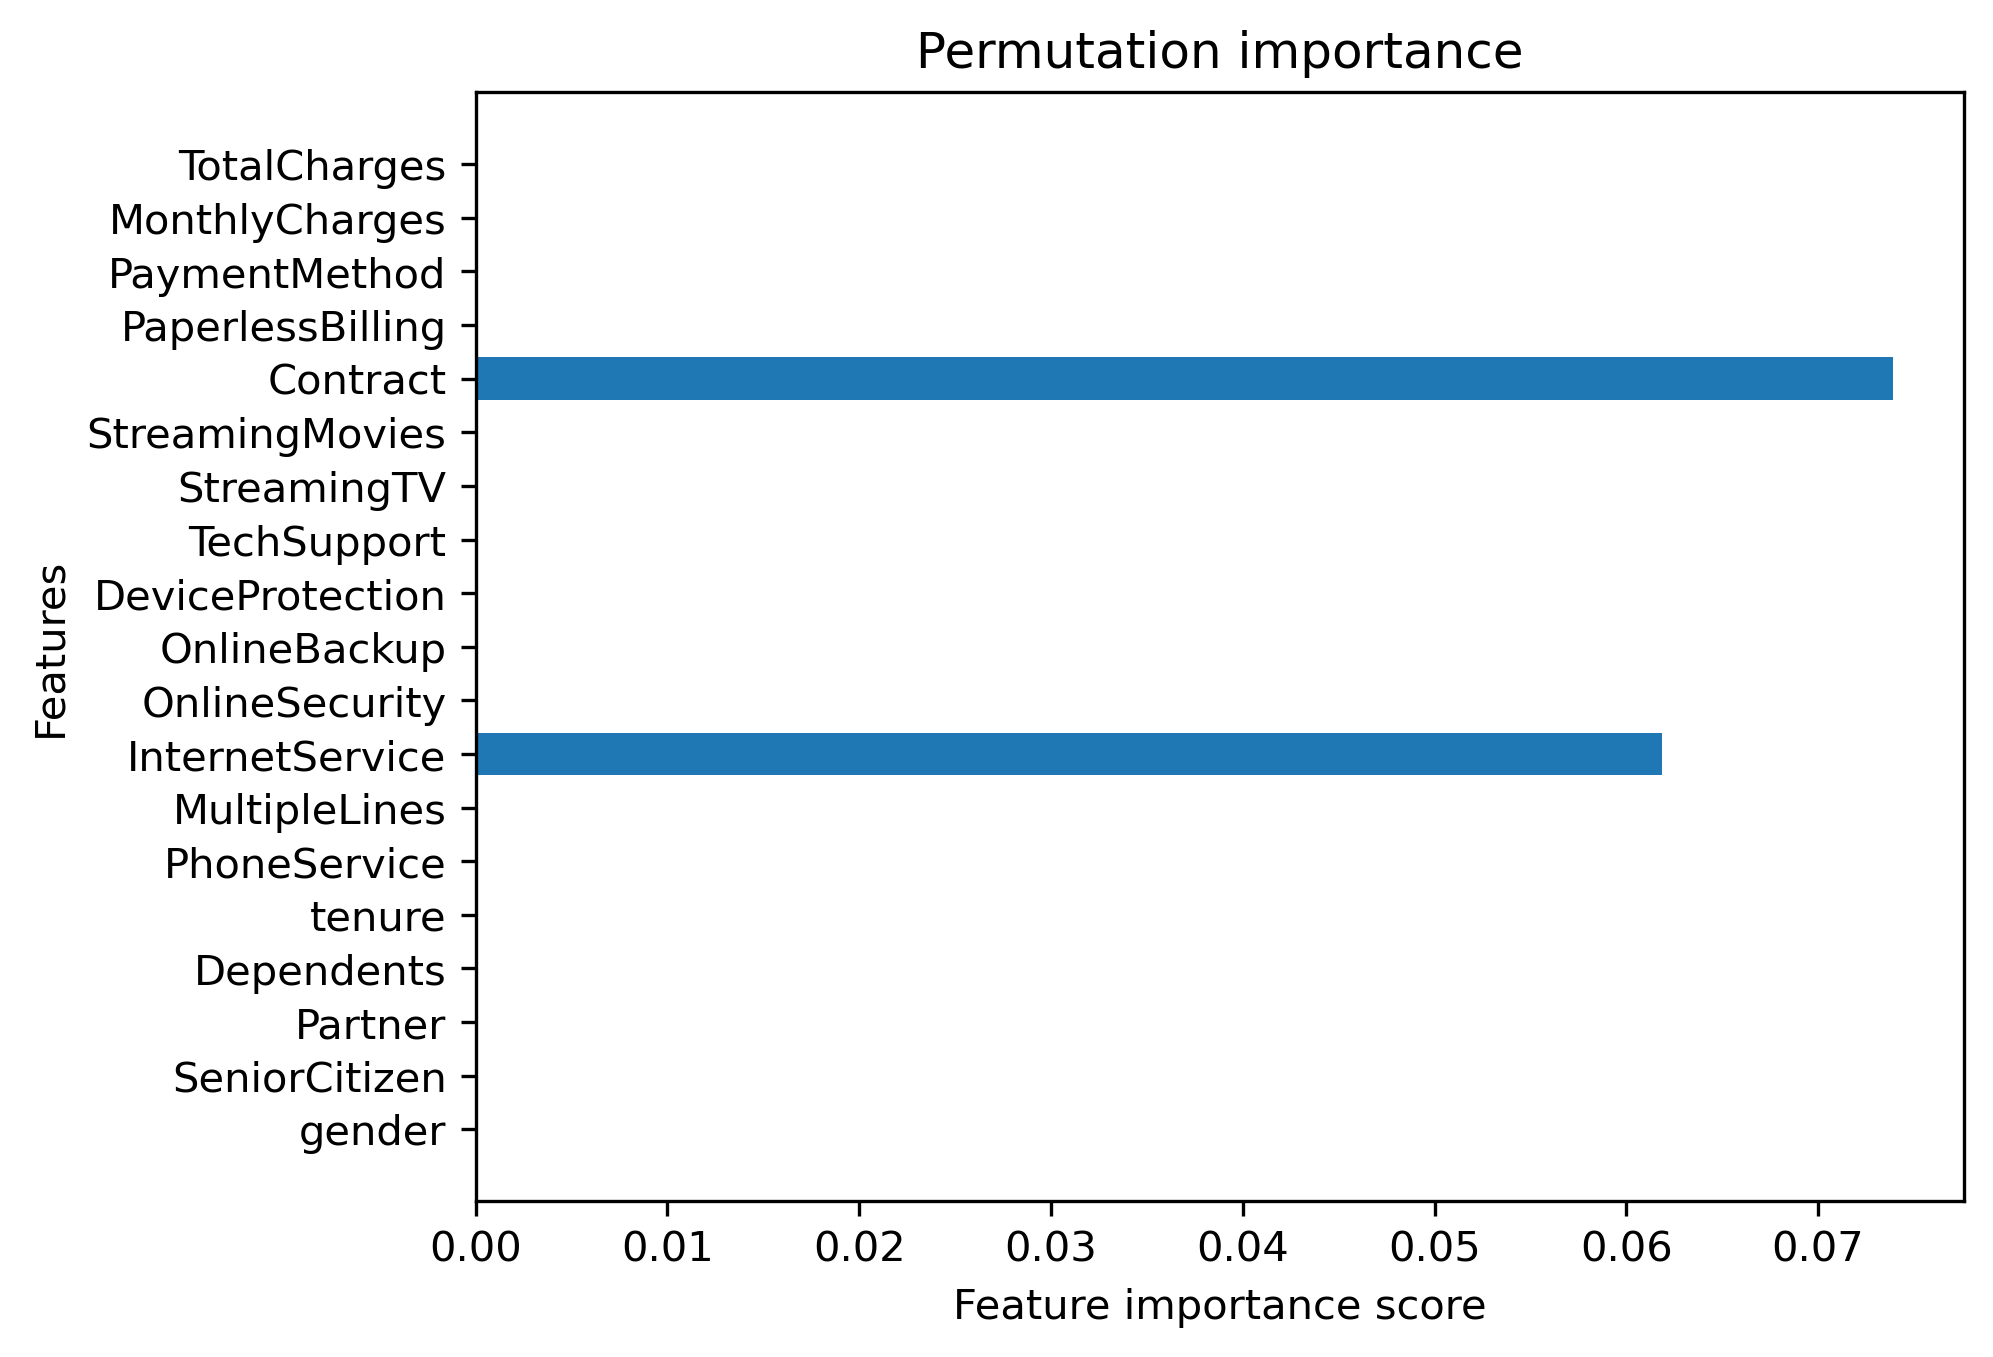
\includegraphics[width=0.8\textwidth]{figures/feature_importance.png}
  \caption{Permutation importance scores of my selected model on the test dataset. 
           The accuracy score was used as performance metric, and each column was
           scrambled 30 times.}
  \label{fig:permutation}
\end{figure}

\paragraph{Score interpretation.} 
The non-zero permutation scores are still very small, 
which means that the model accuracy changes very little when the model cannot rely on the features.
The reason might have to do with how accurate random guesses are compared to predictions.
Let's say the model is in the process of routing a data point, and it reaches a node that routes
based on the scrambled feature.
Since the data point's value of that feature is random,
the direction it will be routed is also random.
In other words, the model prediction is derived using a certain amount of guesswork.
However, random guesses are often accurate in the case of this dataset.
Since the dataset has two possible label types, and 73 \% of the datapoints are labeled \textit{no churn}
in the train dataset,
a baseline model only predicting \textit{no churn} would get a 73 \% accuracy score on that dataset.
My selected decision tree classifier received a 77 \% accuracy score on the test data,
which is not much of an improvement.
This can explain the low permutation scores, because models having to result to 
some naive guesswork still can predict relatively accurately.

\paragraph{Algorithm weakness.}
The barplot in \autoref{fig:permutation} 
illustrates a weakness in this method of finding important features.
The scores indicate that my selected model only uses two features to predict every label.
However, that does not mean that those two features are the only informative ones.
Several of the other features might also carry information, but since they most probably
correlate with the two selected features, they might introduce more noise than information
to models fitted on them.
Therefore, permutation importance scores are not necessarily a good approach for finding
\textit{all} informative features.

\section{Conclusion}

My implementation of the ID3 classifier performs well compared to Sklearn's implementation.
However, it does not perform particularly well on the churn dataset.
My model does not outperform baseline models to a high extent.
It received a recall score of 0.605, which means that it on average only manages to 
correctly classify 61 \% of the \textit{churn} labels. Additionally, its precision score
of 0.565 indicates that 43 \% of its predicted \textit{churn} values are false positives.
The low permutation scores also illustrate how the model's high accuracy score
barely outperforms a baseline model only predicting \textit{no churn} values.
Therefore, it might be wise to utilize other model families to generalize
this dataset.

\section*{On my use of AI}

I have not used AI to generate text or code that I used in this project.
All implementations and reasoning are my own.
AI has only been used for purposes such as understanding the documentation and use cases of methods.
One good example is when I asked Claude how efficient it is to iterate through the rows 
in a pandas dataframe.

\end{document}
